% vim: set textwidth=120:

% Example CV based on the 1.5-column-cv template. Main features:
% * uses the Roboto font family and IcoMoon icon set;
% * doesn't use colours, different font weights are used instead for styling;
% * because the CV fits on one page, header and footer is empty, since there isn't much useful info to put there;
% * includes a photo.
\documentclass[a4paper,10pt]{article}


% package imports
% ---------------

\usepackage[british]{babel} % for correct language and hyphenation and stuff
\usepackage{calc}           % for easier length calculations (infix notation)
\usepackage{enumitem}       % for configuring list environments
\usepackage{fancyhdr}       % for setting header and footer
\usepackage{fontspec}       % for fonts
\usepackage{geometry}       % for setting margins (\newgeometry)
\usepackage{graphicx}       % for pictures
\usepackage{microtype}      % for microtypography stuff
\usepackage{xcolor}         % for colours
\usepackage{datetime}
\usepackage{hyperref}
\usepackage{shadowtext}



% margin and column widths
% ------------------------

% margins
\newgeometry{left=8mm,right=15mm,top=15mm,bottom=15mm}

% width of the gap between left and right column
\newlength{\cvcolumngapwidth}
\setlength{\cvcolumngapwidth}{3.5mm}

% left column width
\newlength{\cvleftcolumnwidth}
\setlength{\cvleftcolumnwidth}{42.5mm}

% right column width
\newlength{\cvrightcolumnwidth}
\setlength{\cvrightcolumnwidth}{\textwidth-\cvleftcolumnwidth-\cvcolumngapwidth}

% set paragraph indentation to 0, because it screws up the whole layout otherwise
\setlength{\parindent}{0mm}


% style definitions
% -----------------
% style categories explanation:
% * \cvnameXXX is used for the name;
% * \cvsectionXXX is used for section names (left column, accompanied by a horizontal rule);
% * \cvtitleXXX is used for job/education titles (right column);
% * \cvdurationXXX is used for job/education durations (left column);
% * \cvheadingXXX is used for headings (left column);
% * \cvmainXXX (and \setmainfont) is used for main text;
% * \cvruleXXX is used for the horizontal rules denoting sections.

% font families
\defaultfontfeatures{Ligatures=TeX} % reportedly a good idea, see https://tex.stackexchange.com/a/37251

% Configure a directory location for fonts(default: 'fonts/')
\newcommand*{\fontdir}[1][fonts/]{\def\@fontdir{#1}}
\fontdir


\newfontfamily{\cvnamefont}{Roboto Medium}
\newfontfamily{\cvsectionfont}{Roboto Medium}
\newfontfamily{\cvtitlefont}{Roboto Regular}
\newfontfamily{\cvdurationfont}{Roboto Light Italic}
\newfontfamily{\cvheadingfont}{Roboto Regular}
\newfontfamily{\cvhonorfont}{Roboto Medium}
\newfontfamily{\cvboldfont}[Path=\@fontdir,Scale=1]{OpenSans-SemiBold}
\newfontfamily{\cvskillfont}[Path=\@fontdir,Scale=1]{OpenSans-SemiBoldItalic}
\setmainfont{Roboto Light}

% colours
\definecolor{cvnamecolor}{HTML}{000000}
\definecolor{cvsectioncolor}{HTML}{3366ff}
\definecolor{cvtitlecolor}{HTML}{000000}
\definecolor{cvdurationcolor}{HTML}{000000}
\definecolor{cvheadingcolor}{HTML}{000000}
\definecolor{cvmaincolor}{HTML}{000000}
\definecolor{cvrulecolor}{HTML}{000000}
\definecolor{cvwhatcolor}{HTML}{5588ff}
\definecolor{cvwherecolor}{HTML}{656565}
\definecolor{cvnoskillcolor}{HTML}{d9d9d9}
\definecolor{cvboldcolor}{HTML}{808080}
\definecolor{cvskilledcolor}{HTML}{668cff}
\color{cvmaincolor}

% styles
\newcommand{\cvnamestyle}[1]{{\Large\cvnamefont\textcolor{cvnamecolor}{#1}}}
\newcommand{\cvsectionstyle}[1]{{\normalsize\cvsectionfont\textcolor{cvsectioncolor}{#1}}}
\newcommand{\cvtitlestyle}[1]{{\large\cvtitlefont\textcolor{cvtitlecolor}{#1}}}
\newcommand{\cvdurationstyle}[1]{{\small\cvdurationfont\textcolor{cvdurationcolor}{#1}}}
\newcommand{\cvheadingstyle}[1]{{\normalsize\cvheadingfont\textcolor{cvheadingcolor}{#1}}}
\newcommand{\cvboldstlye}[1]{{\normalsize\cvboldfont\textcolor{cvboldcolor}{\scalebox{.93}[1.0]{#1}}}}
\newcommand{\cvskillstlye}[1]{{\normalsize\cvskillfont\textcolor{cvwherecolor}{\scalebox{.95}[1.0]{#1}}}}

% Date time format
\newdateformat{monthyeardate}{%
  \THEDAY \space \monthname[\THEMONTH] \THEYEAR}


% inter-item spacing
% ------------------

% vertical space after personal info and standard CV items
\newlength{\cvafteritemskipamount}
\setlength{\cvafteritemskipamount}{5mm plus 1.25mm minus 1.25mm}

% vertical space after other items
\newlength{\cvafterotheritemskipamount}
\setlength{\cvafterotheritemskipamount}{2mm plus 1mm minus 1mm}


% vertical space after sections
\newlength{\cvaftersectionskipamount}
\setlength{\cvaftersectionskipamount}{1mm plus 0.5mm minus 0.5mm}

% extra vertical space to be used when a section starts with an item with a heading (e.g. in the skills section),
% so that the heading does not follow the section name too closely
\newlength{\cvbetweensectionandheadingextraskipamount}
\setlength{\cvbetweensectionandheadingextraskipamount}{1mm plus 0.25mm minus 0.25mm}


% intra-item spacing
% ------------------

% vertical space after name
\newlength{\cvafternameskipamount}
\setlength{\cvafternameskipamount}{3mm plus 0.75mm minus 0.75mm}

% vertical space after personal info lines
\newlength{\cvafterpersonalinfolineskipamount}
\setlength{\cvafterpersonalinfolineskipamount}{2mm plus 0.5mm minus 0.5mm}

% vertical space after titles
\newlength{\cvaftertitleskipamount}
\setlength{\cvaftertitleskipamount}{1mm plus 0.25mm minus 0.25mm}

% value to be used as parskip in right column of CV items and itemsep in lists (same for both, for consistency)
\newlength{\cvparskip}
\setlength{\cvparskip}{0.5mm plus 0.125mm minus 0.125mm}

% set global list configuration (use parskip as itemsep, and no separation otherwise)
\setlist{parsep=0mm,topsep=0mm,partopsep=0mm,itemsep=\cvparskip}


% CV commands
% -----------

% creates a "personal info" CV item with the given left and right column contents, with appropriate vertical space after
% @param #1 left column content (should be the CV photo)
% @param #2 right column content (should be the name and personal info)
\newcommand{\cvpersonalinfo}[2]{
    % left and right column
    \begin{minipage}[t]{\cvleftcolumnwidth}
        \vspace{0mm} % XXX hack to align to top, see https://tex.stackexchange.com/a/11632
        \raggedleft #1
    \end{minipage}% XXX necessary comment to avoid unwanted space
    \hspace{\cvcolumngapwidth}% XXX necessary comment to avoid unwanted space
    \begin{minipage}[t]{\cvrightcolumnwidth}
        \vspace{0mm} % XXX hack to align to top, see https://tex.stackexchange.com/a/11632
        #2
    \end{minipage}

    % space after
    \vspace{\cvafteritemskipamount}
}

% typesets a name, with appropriate vertical space after
% @param #1 name text
\newcommand{\cvname}[1]{
    % name
    \cvnamestyle{#1}

    % space after
    \vspace{\cvafternameskipamount}
}

% typesets a line of personal info beginning with an icon, with appropriate vertical space after
% @param #1 parameters for the \includegraphics command used to include the icon
% @param #2 icon filename
% @param #3 line text
\newcommand{\cvpersonalinfolinewithicon}[3]{
    % icon, vertically aligned with text (see https://tex.stackexchange.com/a/129463)
    \raisebox{.5\fontcharht\font`E-.5\height}{\includegraphics[#1]{#2}}
    % text
    #3

    % space after
    \vspace{\cvafterpersonalinfolineskipamount}
}

% creates a "section" CV item with the given left column content, a horizontal rule in the right column, and with
% appropriate vertical space after
% @param #1 left column content (should be the section name)
\newcommand{\cvsection}[1]{
    % left and right column
    \begin{minipage}[t]{\cvleftcolumnwidth}
        \raggedleft\cvsectionstyle{#1}
    \end{minipage}% XXX necessary comment to avoid unwanted space
    \hspace{\cvcolumngapwidth}% XXX necessary comment to avoid unwanted space
    \begin{minipage}[t]{\cvrightcolumnwidth}
        \textcolor{cvrulecolor}{\rule{\cvrightcolumnwidth}{0.3mm}}
    \end{minipage}

    % space after
    \vspace{\cvaftersectionskipamount}
}

% creates a standard, multi-purpose CV item with the given left and right column contents, parskip set to cvparskip
% in the right column, and with appropriate vertical space after
% @param #1 left column content
% @param #2 right column content
\newcommand{\cvitem}[2]{
    % left and right column
    \begin{minipage}[t]{\cvleftcolumnwidth}
        \raggedleft #1
    \end{minipage}% XXX necessary comment to avoid unwanted space
    \hspace{\cvcolumngapwidth}% XXX necessary comment to avoid unwanted space
    \begin{minipage}[t]{\cvrightcolumnwidth}
        \setlength{\parskip}{\cvparskip} #2
    \end{minipage}

    % space after
    \vspace{\cvafteritemskipamount}
}

\newcommand{\cvhonoritem}[2]{
    % left and right column
    \begin{minipage}[t]{\cvleftcolumnwidth}
        \raggedleft #1
    \end{minipage}% XXX necessary comment to avoid unwanted space
    \hspace{\cvcolumngapwidth}% XXX necessary comment to avoid unwanted space
    \begin{minipage}[t]{\cvrightcolumnwidth}
        \setlength{\parskip}{\cvparskip} #2
    \end{minipage}

    % space after
    \vspace{1.7mm}
}


\newcommand{\cvotheritem}[2]{
    % left and right column
    \begin{minipage}[t]{\cvleftcolumnwidth}
        \raggedleft #1
    \end{minipage}% XXX necessary comment to avoid unwanted space
    \hspace{\cvcolumngapwidth}% XXX necessary comment to avoid unwanted space
    \begin{minipage}[t]{\cvrightcolumnwidth}
        \setlength{\parskip}{\cvparskip} #2
    \end{minipage}

    % space after
    \vspace{\cvafterotheritemskipamount}
}
% typesets a title, with appropriate vertical space after
% @param #1 title text
\newcommand{\cvtitle}[1]{
    % title
    \cvtitlestyle{#1}

    % space after
    \vspace{\cvaftertitleskipamount}
    % XXX need to subtract cvparskip here, because it is automatically inserted after the title "paragraph"
    \vspace{-\cvparskip}
}

% cv Skill Bar
\makeatletter
\newdimen\skillb@level
\newdimen\skillb@length
\newdimen\skillb@height
\skillb@length=89pt%
\skillb@height=8pt%
\newcommand*{\skillbar}[1]{%
    \skillb@level=\dimexpr#1\skillb@length/100\relax%
    {\color{cvskilledcolor}\rule{\skillb@level}{\skillb@height}}%
    {\color{cvnoskillcolor}%
        \rule{\dimexpr\skillb@length-\skillb@level\relax}{\skillb@height}}%

}
\makeatother

% header and footer
% -----------------

% set empty header and footer
\pagestyle{empty}



% preamble end/document start
% ===========================

\begin{document}



% personal info
% -------------

\cvpersonalinfo{
    % photo
    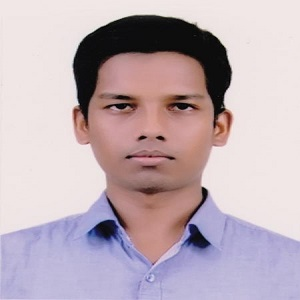
\includegraphics[height=43.5mm]{Sizan.jpg}
    }{
    % name
    \cvname{\textbf{}}
    \cvname{\textbf{MD. OLIULLAH SIZAN}}
    % \cvname\textcolor{}{\textbf{MD. OLIULLAH SIZAN}}

    % address
    \cvpersonalinfolinewithicon{height=4mm}{072-location.pdf}{
        144/12, Mukti Housing, South Pirerbag, Mirpur, Dhaka-1216, Bangladesh
    }

    % phone number
    \cvpersonalinfolinewithicon{height=4mm}{067-phone.pdf}{
        {\cvskillstlye{{+880 1781-443195} \textbar\space {+880 1518-456575}}
    }}

    % email address
    \cvpersonalinfolinewithicon{height=4mm}{070-envelop.pdf}{
        \href{mailto:mdoliullahsizan5@gmail.com}{mdoliullahsizan5@gmail.com}
    }

    % LinkedIn account
    \cvpersonalinfolinewithicon{height=4mm}{458-linkedin.pdf}{
        \href{https://www.linkedin.com/in/md-oliullah-sizan-00364b140/}{md-oliullah-sizan-00364b140}
    }

    % GitHub account
    \cvpersonalinfolinewithicon{height=4mm}{github1.png}{
        \href{https://github.com/mdoliullahsizan}{mdoliullahsizan}
    }
    
    % % Skype account
    % \cvpersonalinfolinewithicon{height=4mm}{skype.jpg}{
    %     \href{https://www.skype.com/en/}{live:oliullahsizan5}
    % }
    % DoB:  05\textsuperscript{th} May 1996
    {DoB: May 05, 1996}

    % % DoB
    % \cvpersonalinfolinewithicon{height=4mm}{dob1.jpg}{
    %     \href{https://github.com/mdoliullahsizan}{05\textsuperscript{th} May 1996}
    % }
   
    
}

% education
% ---------



\cvsection{\textbf{WORK EXPERIENCES}}

\vspace{\cvbetweensectionandheadingextraskipamount}

% Work Exp 01
\cvhonoritem{
    \cvdurationstyle{Dec 2019 -- Present}
    }
{
     \cvtitlestyle{Junior Officer} \textcolor{cvwherecolor}{\textbf{\textbar}} \emph{bKash Care (Back Office)} \cvdurationstyle{@}
  \textcolor{cvwhatcolor}{\emph{\textbf{{bKash Ltd}}}}
}

% % Work Exp 02
% \cvhonoritem{
%     \cvdurationstyle{Oct 2019 -- Nov 2019}
%     }
% {
%     \cvtitlestyle{Support Engineer} \textcolor{cvwherecolor}{\textbf{\textbar}} \emph{Trainee} \cvdurationstyle{@} 
%     \textcolor{cvwhatcolor}{\emph{\textbf{Zara Zaman Technology Ltd}}}
% }






\cvsection{\textbf{EDUCATION}}



% bachelor's
\cvitem{
    \cvdurationstyle{April 2015 -- August 2019}
}{
    \cvtitle{Bachelor of Science (B.Sc.) in Computer Science \& Engineering}

     \textcolor{cvwhatcolor}{\emph{\textbf{CGPA: 2.65}}}
    \textcolor{cvwherecolor}{\textbf{\textbar}}
    \textcolor{cvwherecolor}{\emph{\textbf{City University, Bangladesh}}}
    \textcolor{cvwherecolor}{\textbf{\textbar}}
     \textcolor{cvwherecolor}{\emph{\textbf{Dhaka}}}
    }

%     \begin{itemize}[leftmargin=*]
%         \item Interest Areas: \emph{Machine Design, CAD/CAE, Strength of Materials, Numerical Computation}
%         \item Member - SPCE Racing \textbf{\textbar}\space Society of Automotive Engineers India Collegiate Club 
%         \item Head - Operations \& Logistics \textbf{\textbar}\space SPACE '16 (College Cultural Festival) 
%         \item Secretary \textbf{\textbar}\space IEEE-SPCE-SPIT Student Association, 2014-15 
%         \item Co-Head - Performing Arts \textbf{\textbar} \space SPACE '15 (College Cultural Festival)
%     \end{itemize}
% }

% higher secondary schooling
\cvitem{
    \cvdurationstyle{August 13, 2014 }
}{
    \cvtitle{Higher Secondary Certificate in Science}

    \textcolor{cvwhatcolor}{\emph{\textbf{CGPA: 3.70}}}
    \textcolor{cvwherecolor}{\textbf{\textbar}}
    \textcolor{cvwherecolor}{\emph{\textbf{Mohammadpur Model School \& College}}}
     \textcolor{cvwherecolor}{\textbf{\textbar}}
     \textcolor{cvwherecolor}{\emph{\textbf{Dhaka}}}

    % \begin{itemize}[leftmargin=*]
    %     \item Subjects: Physics, Chemistry, Mathematics \& Statistics, Electronics(Analog \& Digital)
    %     \item Among the Top 1\% candidates passing the Class XII State Board Examination
    %     \item Secured 1\textsuperscript{st} Rank in Class XI among 135 students
    % \end{itemize}
}
% schooling 
\cvitem{
    \cvdurationstyle{May 07, 2012}
}{
    \cvtitle{Secondary School Certificate in Science}

    \textcolor{cvwhatcolor}{\emph{\textbf{CGPA: 4.50}}}
    \textcolor{cvwherecolor}{\textbf{\textbar}}
    \textcolor{cvwherecolor}{\emph{\textbf{Sher-E-Bangla Nagar Govt. Boys' High School}}}
     \textcolor{cvwherecolor}{\textbf{\textbar}}
     \textcolor{cvwherecolor}{\emph{\textbf{Dhaka}}}


    % \begin{itemize}[leftmargin=*]
    %     \item Part of the School's Music Club, Football Team (Under 16/14/12/10) and Boy Scouts Guild
    % \end{itemize}
}

% % Projects Undertaken
% %-------

% \cvsection{\textbf{PROJECTS}}

% \vspace{\cvbetweensectionandheadingextraskipamount}

% % project 1
% \cvitem{
%     \cvdurationstyle{July 2016 -- April 2017}
%     }
% {
%     \cvtitle{Design and Development of an Automatic Torque Biasing Differential (ATBD)}
%     \textcolor{cvwhatcolor}{\emph{\textbf{{B. Tech. Final Year Project}}}}
%     \textcolor{cvwherecolor}{\textbf{\textbar}}
%     \textcolor{cvwherecolor}{\emph{\textbf{Sardar Patel College of Engineering, Mumbai}}}   

%     \begin{itemize}[leftmargin=*]
%         \item Involved {\cvboldstlye{Mathematical Modelling}} of a {\cvboldstlye{Double Helical Planetary Gear System}} based ATBD
%         \item {\cvboldstlye{Optimization of involute gear geometry }}was carried out to produce a compact design
%         \item Parametric CAD model assembly was created using variables and expressions in \emph{CATIA v5}  
%         \item Detail design of individual components was performed using Machine Design Handbooks
%         \item {\cvboldstlye{Performed Finite Element Analysis}} to validate design calculations in \emph{ANSYS Mechanical}
%         \item Manufacturing process for components was developed and mock-up assembly was built to depict a proof of concept
       
%     \end{itemize}

% }
% % project 2
% \cvitem{
%     \cvdurationstyle{January 2017 -- March 2017}
%     }
% {
%     \cvtitle{Design of an Electric Overhead Travelling (EOT) Crane}
%         \textcolor{cvwhatcolor}{\emph{\textbf{{Design of Mechanical Systems Course Project}}}}
%         \textcolor{cvwherecolor}{\textbf{\textbar}}
%         \textcolor{cvwherecolor}{\emph{\textbf{Sardar Patel College of Engineering, Mumbai}}}

%     \begin{itemize}[leftmargin=*]
%         \item {\cvboldstlye{Designed a 20-ton SWL, 24-metre span EOT Crane}} based on IS 13834/ISO 4301 \& IS 3177 within the scope of girders, trolley, wheels, rope drum, rope, snatch block and hook  
%         \item {\cvboldstlye{Fabrication drawings}} were created in \emph{CATIA v5} and critical components analysed in \emph{ANSYS}
%         \item Along with a 4-member team, obtained the {\cvboldstlye{highest score of \emph{18/20}}} for the proposal   
%     \end{itemize}
%}



% \cvsection{\textbf{ACCOLADES}}

% \vspace{\cvbetweensectionandheadingextraskipamount}

% % Award 1
% \cvhonoritem{
%     \cvdurationstyle{November 2018}
%     }
% {
%      \cvtitlestyle{Winner - TECHiQ Contest} \textcolor{cvwherecolor}{\textbf{\textbar}} \emph{for the most technologically sound 6-member team among 1400+ employees across all L\&T Defence locations} \cvdurationstyle{@}
%   \textcolor{cvwhatcolor}{\emph{\textbf{{Larsen \& Toubro Limited, Mumbai}}}}
% }


% % Award 2
% \cvhonoritem{
%     \cvdurationstyle{June 2017}
%     }
% {
%     \cvtitlestyle{Cognizant Best Outgoing Student Award 2017} \textcolor{cvwherecolor}{\textbf{\textbar}} \emph{for academic and extra-curicular performance among 230+ graduating pupils} \cvdurationstyle{@} 
%     \textcolor{cvwhatcolor}{\emph{\textbf{Sardar Patel College of Engineering, Mumbai}}}
% }

% % Award 3
% \cvitem{
%     \cvdurationstyle{July 2016}
%     }
% {
%     \cvtitlestyle{Go Green Award \& 7th Place Overall - SPCE Racing} \textcolor{cvwherecolor}{\textbf{\textbar}} \emph{for the most fuel efficient car and cumulative points secured among 172 teams} \cvdurationstyle{@}
%     \textcolor{cvwhatcolor}{\emph{\textbf{{SUPRA SAEINDIA 2016}}}}
% }


\cvsection{\textbf{ACTIVITIES \& PARTICIPATION}}

\vspace{\cvbetweensectionandheadingextraskipamount}

% ACTIVITIES 01
\cvhonoritem{
    \cvdurationstyle{Feb 2019 -- Aug 2019}
    }
{
     \cvtitlestyle{Mentor} \textcolor{cvwherecolor}{\textbf{\textbar}} \emph{City University Computer Club (CUCC)} \cvdurationstyle{@}
  \textcolor{cvwhatcolor}{\emph{\textbf{{City University, Bangladesh}}}}
}
% ACTIVITIES 02
\cvhonoritem{
    \cvdurationstyle{Jan 2016 -- Jan 2019}
    }
{
    \cvtitlestyle{Member} \textcolor{cvwherecolor}{\textbf{\textbar}} \emph{City University Programming Club (CUPC)} \cvdurationstyle{@} 
    \textcolor{cvwhatcolor}{\emph{\textbf{City University, Bangladesh}}}
}

% ACTIVITIES 03
\cvitem{
    \cvdurationstyle{2018}
    }
{
    \cvtitlestyle{Volunteer} \textcolor{cvwherecolor}{\textbf{\textbar}} \emph{(MOVers)} \cvdurationstyle{@}
    \textcolor{cvwhatcolor}{\emph{\textbf{Bangladesh Mathematical Olympiad}}}
}

% % ACTIVITIES 04
% \cvitem{
%     \cvdurationstyle{2018}
%     }
% {
%     \cvtitlestyle{Member} \textcolor{cvwherecolor}{\textbf{\textbar}} \emph{Google Crowdsource Bangladesh Community } \cvdurationstyle{@}
%     \textcolor{cvwhatcolor}{\emph{\textbf{City University, Bangladesh}}}
% }

% % PARTICIPATION 05
% \cvitem{
%     \cvdurationstyle{Feb 2018}
%     }
% {
%     \cvtitlestyle{Enumerator} \textcolor{cvwherecolor}{\textbf{\textbar}} \emph{National Household Database (NHD) Project 2018} \cvdurationstyle{@}
%     \textcolor{cvwhatcolor}{\emph{\textbf{{Bangladesh Bureau of Statistics (BBS)}}}}
% }

% % PARTICIPATION 06
% \cvitem{
%     \cvdurationstyle{May 2017}
%     }
% {
%     \cvtitlestyle{Participant} \textcolor{cvwherecolor}{\textbf{\textbar}} \emph{IoT Conference 2017} \cvdurationstyle{@}
%     \textcolor{cvwhatcolor}{\emph{\textbf{{Bangladesh Innovation Forum (BIF)}}}}
% }

% % PARTICIPATION 07
% \cvitem{
%     \cvdurationstyle{April 2017}
%     }
% {
%     \cvtitlestyle{Participant} \textcolor{cvwherecolor}{\textbf{\textbar}} \emph{National Power \& Energy Hackathon 2017} \cvdurationstyle{@}
%     \textcolor{cvwhatcolor}{\emph{\textbf{{Ministry of Power, Energy \& Mineral Resources, Bangladesh}}}}
% }


% \cvsection{\textbf{PARTICIPATION}}

% \vspace{\cvbetweensectionandheadingextraskipamount}

% % % PARTICIPATION 01
% % \cvhonoritem{
% %     \cvdurationstyle{June 2019}
% %     }
% % {
% %      \cvtitlestyle{Enumerator} \textcolor{cvwherecolor}{\textbf{\textbar}} \emph{Agricultural Survey 2019} \cvdurationstyle{@}
% %   \textcolor{cvwhatcolor}{\emph{\textbf{{Bangladesh Bureau of Statistics (BBS)}}}}
% % }


% PARTICIPATION 02
\cvhonoritem{
    \cvdurationstyle{Dec 2018}
    }
{
    \cvtitlestyle{Java} \textcolor{cvwherecolor}{\textbf{\textbar}} \emph{Top-up IT Training} \cvdurationstyle{@} 
    \textcolor{cvwhatcolor}{\emph{\textbf{Bangladesh Computer Council (BCC)}}}
}

% % PARTICIPATION 03
% \cvitem{
%     \cvdurationstyle{Feb 2018}
%     }
% {
%     \cvtitlestyle{Enumerator} \textcolor{cvwherecolor}{\textbf{\textbar}} \emph{National Household Database (NHD) Project 2018} \cvdurationstyle{@}
%     \textcolor{cvwhatcolor}{\emph{\textbf{{Bangladesh Bureau of Statistics (BBS)}}}}
% }

% PARTICIPATION 04
\cvitem{
    \cvdurationstyle{May 2017}
    }
{
    \cvtitlestyle{Participant} \textcolor{cvwherecolor}{\textbf{\textbar}} \emph{IoT Conference 2017} \cvdurationstyle{@}
    \textcolor{cvwhatcolor}{\emph{\textbf{{Bangladesh Innovation Forum (BIF)}}}}
}

% % PARTICIPATION 05
\cvitem{
    \cvdurationstyle{April 2017}
    }
{
    \cvtitlestyle{Participant} \textcolor{cvwherecolor}{\textbf{\textbar}} \emph{National Power \& Energy Hackathon 2017} \cvdurationstyle{@}
    \textcolor{cvwhatcolor}{\emph{\textbf{{Ministry of Power, Energy \& Mineral Resources, Bangladesh}}}}
}



% skills
% ------

\cvsection{\textbf{SKILLS}}

\vspace{\cvbetweensectionandheadingextraskipamount}


% OS
\vspace{-2mm}
\cvitem{
    \cvheadingstyle{Operating System}
    
}{  
        \setlength\tabcolsep{5pt}
        \begin{tabular}{|l|l|}
       Windows & Ubuntu \\
        %  \skillbar{80} & \skillbar{40} \\
        %  \footnotesize{\emph{}} &
        %  \footnotesize{\emph{Ubuntu}} \\
        \end{tabular}
 }


% MS Office
\vspace{-2mm}
\cvitem{
    \cvheadingstyle{MS Office}
    
}{  
        \setlength\tabcolsep{5pt}
        \begin{tabular}{|l|l|l|}
        Word & PowerPoint & Excel \\
        %  \skillbar{70} & \skillbar{50} & \skillbar{60}\\
        %  \footnotesize{\emph{350+ hours of practice}} & \footnotesize{\emph{200+ hours of practice}} & \footnotesize{\emph{100+ hours of practice}}\\
        \end{tabular}
 } 



% % Prog Lang
% \cvitem{
%     \cvheadingstyle{Programming Language}
    
% }{  
%         \setlength\tabcolsep{5pt}
%         \begin{tabular}{|l|l|l|}

%         Java & C \\
%         % \skillbar{40} & \skillbar{30} & \skillbar{50} \\
%         % \footnotesize{\emph{350+ hours of experience}} & \footnotesize{\emph{200+ hours of experience}} & \footnotesize{\emph{250+ hours of experience}} & \footnotesize{\emph{300+ hours of experience}}\\
%         \end{tabular}
    
%     % \begin{itemize}[leftmargin=4mm]
%     % \normalsize
%     %     \item{Completed an {\cvboldstlye{80-hour Certification Course on CATIA v5}} from CADD Centre}
%     %     \item{Received on-the-job training for Siemens NX and HyperMILL at Larsen \& Toubro Limited}
%     % \end{itemize}
% }



% Prog & Sripting Lang
\cvitem{
    \cvheadingstyle{Programming \& Scripting Language, Database}
    
}{  
        \setlength\tabcolsep{5pt}
        \begin{tabular}{|l|l|l|l|l|l|}

        Java & C & HTML & CSS & JavaScript & MySQL \\
        % \skillbar{40} & \skillbar{30} & \skillbar{50} \\
        % \footnotesize{\emph{350+ hours of experience}} & \footnotesize{\emph{200+ hours of experience}} & \footnotesize{\emph{250+ hours of experience}} & \footnotesize{\emph{300+ hours of experience}}\\
        \end{tabular}
    
    % \begin{itemize}[leftmargin=4mm]
    % \normalsize
    %     \item{Completed an {\cvboldstlye{80-hour Certification Course on CATIA v5}} from CADD Centre}
    %     \item{Received on-the-job training for Siemens NX and HyperMILL at Larsen \& Toubro Limited}
    % \end{itemize}
}





% % Scripting Lang
% \vspace{-2mm}
% \cvitem{
%     \cvheadingstyle{Scripting Language}
    
% }{  
%         \setlength\tabcolsep{5pt}
%         \begin{tabular}{|l|l|l|}
%         HTML & CSS & JavaScript \\
%         %  \skillbar{65} & \skillbar{60} &  \skillbar{50} & \skillbar{30} \\
%         %  \footnotesize{\emph{350+ hours of practice}} & \footnotesize{\emph{200+ hours of practice}} & \footnotesize{\emph{100+ hours of practice}}\\
%         \end{tabular}
%  }       


% Database
% \vspace{-2mm}
% \cvitem{
%     \cvheadingstyle{Database}
    
% }{  
%         \setlength\tabcolsep{5pt}
%         \begin{tabular}{|l|}
%         MySQL \\
%         %  \skillbar{30} \\
%         %  \footnotesize{\emph{350+ hours of practice}} & \footnotesize{\emph{200+ hours of practice}} & \footnotesize{\emph{100+ hours of practice}}\\
%         \end{tabular}
%  } 
 
 
 
% languages
\vspace{-2mm}
\cvitem{
    \cvheadingstyle{Languages}
    
}{  
        \setlength\tabcolsep{5pt}
        \begin{tabular}{|l|l|}
       Bengali & English \\
        %  \skillbar{100} & \skillbar{70} \\
         \footnotesize{\emph{Mother Tongue}} & \footnotesize{\emph{Good Fluency}} 
         \\
        \end{tabular}
 }
 

% Soft Skills
\vspace{-2mm}
\cvitem{
\cvheadingstyle{Key Skills}
}{\cvskillstlye{{Continuous Learning} \textbar\space {Leadership} \textbar\space {Adaptability} \textbar\space {Networking}  \textbar\space {Interpersonal Skills}}
}

% additional info
% ---------------

\cvsection{\textbf{ADDITIONAL DETAILS}}

\vspace{\cvbetweensectionandheadingextraskipamount}

% interests
\cvotheritem{
   \cvheadingstyle{Hobbies \& Interests}
}{
    \emph{Travelling, Watching Movies, Listening to Music, Reading Books; Playing Cricket, Football}
}
\vspace{3mm}

%\cvsection{\textbf{REFERENCES}}

%\vspace{\cvbetweensectionandheadingextraskipamount}

% interests


% \cvotheritem{
% \cvheadingstyle{}
% }{
% \setlength\tabcolsep{5pt}
% \def\arraystretch{1.4}
% \begin{tabular}{l l l}
%   {\emph{Dr Nilesh Raykar }} & -\space nilesh\_raykar@spce.ac.in & \space\space+91 22 2623 2192  ext. 245 \\
%   {\emph{Dr Kiran Bhole}} & -\space kiran\_bhole@spce.ac.in & \space\space+91 98 6937 8873
% \end{tabular}
% }


% \cvsection{\textbf{}}



% References
% ---------------

\cvsection{\textbf{REFERENCES}}

\vspace{\cvbetweensectionandheadingextraskipamount}

% languages
\vspace{-2mm}
\cvitem{
    \cvheadingstyle{}
    
} {  
        \setlength\tabcolsep{5pt}
        \begin{tabular}{|l|l|}
      Sabbir Muhammad Saleh & Md. Ataullah Bhuiyan \\
        \footnotesize{\emph{Assistant Professor}} & \footnotesize{\emph{Senior Lecturer}} \\
         \footnotesize{\emph{City University, Bangladesh}} & \footnotesize{\emph{City University, Bangladesh}} \\
         % phone number
         \footnotesize{\emph { \cvpersonalinfolinewithicon{height=4mm}{067-phone.pdf}{
        \cvboldstlye{+880 1835-150865}
        }}} &
        % phone number
        \footnotesize{\emph{\cvpersonalinfolinewithicon{height=4mm}{067-phone.pdf}{
        \cvboldstlye{+880 1843-906686}
        }}} \\

     % email address
        \footnotesize{\emph{{\cvpersonalinfolinewithicon{height=4mm}{070-envelop.pdf}{
        \cvboldstlye{ \href{mailto:saleh.sabbir.aiub@gmail.com}{saleh.sabbir.aiub@gmail.com}}}}} }
        &
        % email address
        \footnotesize{\emph { {\cvpersonalinfolinewithicon{height=4mm}{070-envelop.pdf}{
        \cvboldstlye{ \href{mailto:abab_bn@yahoo.com}{abab\_bn@yahoo.com}}}}}} \\
        
        \end{tabular}
 }
 
 

% References
% ---------------

\vspace{0.3cm}


% \begin{itemize}[leftmargin=3mm]
%     \item[] \normalsize Place, Date: \emph{Mumbai, \monthyeardate\today}
%     \item[] {Signature: \cvpersonalinfolinewithicon{height=13mm}{signature.png}{}
%     }
% \end{itemize}




\end{document}




